\chapter{Authentication Mechanisms}
\label{cha:authentication_mechanisms}
This chapter explains the concepts and details of the two compared authentication mechanisms.
Only the mTLS approach and the authentication using self-signed JWTs approach are discussed in this chapter since the Trust the Network (TTN) approach is deprecated and should not be used anymore~\cite{dias2020microservices}.

\begin{figure}
	\centering
	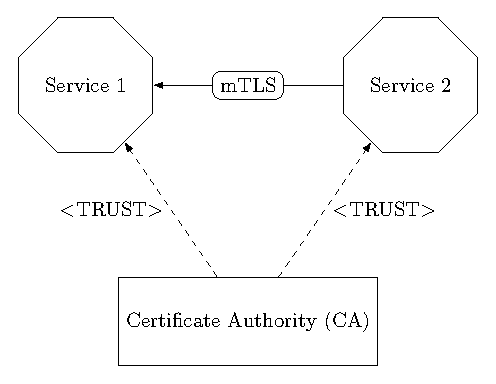
\includegraphics{images/authentication-mechanisms/TikZ_mTLS_base_structure.pdf}
	\caption{Setup using mTLS for the service-to-service authentication~\cite{dias2020microservices}}
	\label{fig:auth_mechanisms_mtls}
\end{figure}

\section{Authentication based on mTLS}
Mutual TLS is the most popular option for the service-to-service authentication of microservice deployments~\cite{dias2020microservices}.
Securing the communication with TLS already provides integrity confidentiality and authenticates the server to the client.
Since TLS does not provide authentication from the client to the server, it is insufficient for service-to-service security.
Therefore mutual TLS is used, which provides an efficient and straightforward approach to authenticating the client to the server.

The authentication using mTLS requires a PKI, the same as TLS on the internet.
It is possible to use the already existing PKI of the internet, but this would make the key management much harder and would not bring any advantages.
% TODO: Insert Reference to self-hosted PKI
Therefore it is good practice to use a self-hosted PKI to have a root of trust within the network~\cite{dias2020microservices}.
The setup of a microservice deployment using mTLS is shown in figure~\ref{fig:auth_mechanisms_mtls}.

When mTLS is used, the server and the client must provide a valid certificate to create a communication channel.
The issuer of the presented certificates must be trusted by all communicating parties~\cite{dias2020microservices}.
If one communication partner does not have a valid certificate, the communication is neglected.
Therefore each service needs its private key and the corresponding public key.
Additionally, a signed certificate, which binds the public key to the certificate's subject, is needed.
The certificates of the communication partners are exchanged during the TLS handshake.

This mechanism can also be used to authenticate the end-users of an application.
The term Client Certificate Authentication (CCA) is used for this context.
The service-to-service authentication using mTLS is an implementation of CCA, but in this approach, the client is not the end-user, instead, it is another service.

\subsection{Handshake}
\label{sec:tlshandshake_details}
The handshake is used to exchange the certificates of the participants and set up the connection.
The handshake steps differ between the used algorithms and versions of the TLS protocol.
The following sequence and figure~\ref{fig:tlshandshake} should give an overview about the steps of the TLS handshake using mutual TLS~\cite{parsovs2013practical}:
\begin{enumerate}
	\item The client initializes the connection by sending a \textbf{ClientHello} message to the server.
		The \textbf{ClientHello} message includes a list of supported cipher suites, and the randomness, which is a combination of random bytes and the current date~\cite{mediumtls}.
	\item The server responds with a \textbf{ServerHello}, in which he chooses one cipher suite of the \textbf{ClientHello} message.
		Furthermore, the \textbf{ServerHello} contains the server's randomness.
	\item The server sends the \textbf{Certificate} messages, containing one or more certificates, which can be used to build the certificate chain.
		The client validates the sent certificates with his own trusted store.
		If it trusts the sent certificate chain, the server is successfully authenticated.
	\item The server sends the \textbf{CertificateRequest} message, in which the trusted CAs of the server are listed.
		The client can use this list to choose the correct certificate he has to present.
	\item The server sends the \textbf{ServerHelloDone} message.
	\item The client responds with his \textbf{Certificate} message, which is similar to the servers \textbf{Certificate} message, but contains the client's certificate chain.
	\item The client then generates a random value for the pre-master secret.
		The pre-master secret derives symmetric keys for the cryptographic operations defined in the cipher suite.
		Then the pre-master secret is encrypted using the server's public key.
		Therefore, only the owner of the corresponding private key, the server, can decrypt this message.
		In the end, the encrypted pre-master secret is transferred to the server within the \textbf{ClientKeyExchange} message.
	\item The client has to prove that he owns the corresponding private key of the certificate he sent.
		Therefore he has to encrypt the hash of all previous messages with his private key.
		This encrypted hash is then sent to the server within the \textbf{CertificateVerify} message.
		The server can decrypt the hash with the certificate's public key and can calculate the hash on its own to check whether the decrypted hash is correct or not.
	\item The client sends a \textbf{ChangeCipherSpec} message to signal the server that all following messages will be protected with the protection mechanisms defined in the cipher suite.
	\item The last message of the handshake is the \textbf{Finished} message, which is an encrypted hash of all previous messages.
	\item Same as step 9, but from the server.
	\item Same as step 10, but from the server.
\end{enumerate}
After the handshake, both participants know the secret, which can encrypt and decrypt messages.
The handshake would have almost the same steps when mTLS is not used.
Only the \textbf{CertificateRequest} message of the sever and the \textbf{Certificate} message and the \textbf{CertificateVerify} message of the client are unique for mTLS.
One special case of the handshake is that the client responds to the \textbf{CertificateRequest} with an empty \textbf{Certificate} message.
Depending on the configuration of the server, the connection without a certificate can be allowed or neglected~\cite{parsovs2013practical}.

\begin{figure}
	\centering
	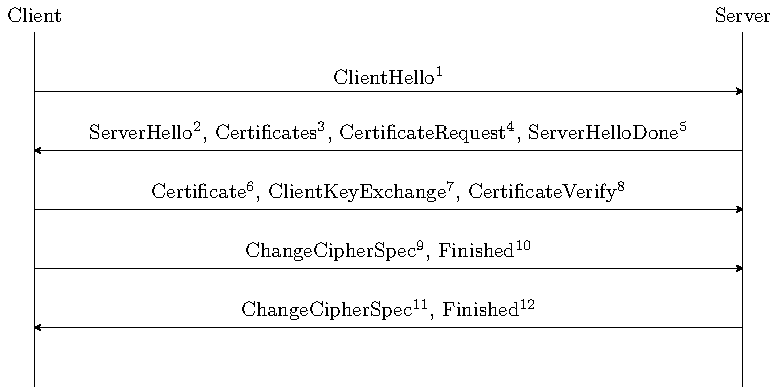
\includegraphics{authentication-mechanisms/TikZ_handshake.pdf}
	\caption{TLS handshake using mTLS~\cite{parsovs2013practical}}
	\label{fig:tlshandshake}
\end{figure}

\subsection{Passing the end user context} \label{sec:mtls_end_user_context}
For some functionalities, the identity of the microservice is not relevant. Instead, the identity of the end-user is relevant.
In those cases, the microservices have to pass the end-user context when they consume the logic of other microservices.
The most popular approach for passing the end-user context with mTLS is JSON Web Tokens.
The JWTs can be embedded within the HTTP Request body or using URL parameters.
This approach can be implemented in multiple ways~\cite{dias2020microservices}.

Generally, the user obtains an access token from any token service.
This token could be an OAuth2, OpenID Connect, or any other token.
The user has to send this token with each request.
The token is then validated by a Security Token Service (STS).
If the token is valid, the STS returns a JWT, which can then be used to consume other services.
When one microservice calls another microservice, he sends the JWT, and if this microservice has to consume another microservice, he also passes the same token to the next microservice~\cite{dias2020microservices}.
The workflow of this approach is shown in figure~\ref{fig:mtls_id_1}
\begin{figure}
	\centering
	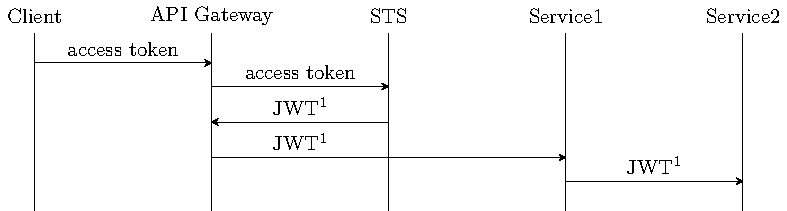
\includegraphics{images/authentication-mechanisms/TikZ_jwt_identity_1.pdf}
	\caption{Use the same JWT for each request~\cite{dias2020microservices}}
	\label{fig:mtls_id_1}
\end{figure}

Another approach is that the STS is used to generate a new token for each request which is shown in figure~\ref{fig:mtls_id_2}.
When the STS generates a new token for each request, he fully knows all performed requests.
Therefore the STS could implement further authorization logic~\cite{dias2020microservices}.
Nevertheless, the frequent calls could result in an enormous workload for the STS and decrease the system's performance.

\begin{figure}[H]
	\centering
	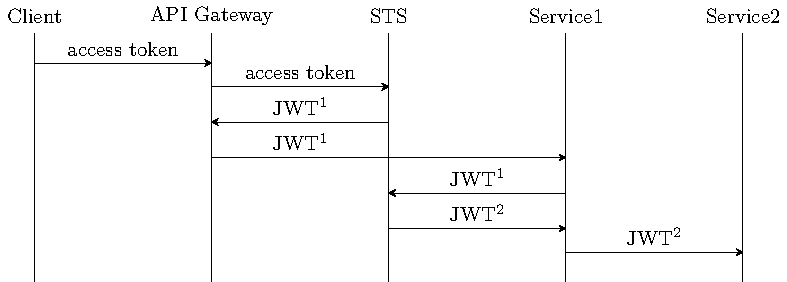
\includegraphics{images/authentication-mechanisms/TikZ_jwt_identity_2.pdf}
	\caption{Generate new JWT for each request~\cite{dias2020microservices}}
	\label{fig:mtls_id_2}
\end{figure}

Both approaches result in some overhead, especially the second one.
Additionally, when the microservices are located in different trust domains, those approaches can get very complicated since a microservice only trusts the STS within its trust domain~\cite{dias2020microservices}.
Therefore, mTLS might not be the superior mechanism for systems that require the end-user context.

\subsection{Conclusion}
mTLS is an efficient mechanism to implement service-to-service authentication.
Since the communication between the services is usually done using HTTPS, the services already use TLS.
Therefore, mTLS does not cause much configuration overhead, and no new technologies are necessary~\cite{dias2020microservices}, unless the services share the end-user context.

One crucial advantage of the TLS handshake is that the private keys are never exchanged, and the session keys are always different due to the usage of the randomness.
This means that even if an intruder can get the session key of a communication channel, he cannot use this key for another session.
Furthermore, it is not possible to retrieve any information about the private key of the communication partners with the knowledge of the session key.
This shows how secure mTLS is, even for advanced attacks~\cite{parsovs2013practical}.

From the developer's perspective, mTLS does not require much implementation logic.
The service which acts as the server has to be configured to use certificate authentication.
Depending on the used technologies, this is usually done by setting a few configuration parameters in the code or directly on the webserver.
The service which acts as the client has to be configured to send his certificate during the TLS handshake.
Most HTTP Client libraries support simply attaching the certificate to each HTTP Request.
Nevertheless, the developers do not have to implement much logic resulting in the problem that they do not have much control over the system.
The developers have to rely on the implementation of the webserver developers.
This means that if a web server has security-related bugs, the microservice developers can not solve them independently.
For example, the apache webserver, one of the most popular webservers, had many issues in combination with CCA.
Arnis Parsovs~\cite{parsovs2013practical} researched the problems of the apache webserver and gave an extensive guide on how to circumvent all bugs when CCA is configured.

% TODO: Referenz auf key management
The biggest challenge of mTLS is the key management, which was described in more detail in the chapter.
Key management is responsible for key provisioning, key revocation, key rotation, and more management tasks.
Usually, the key management requires a self-hosted PKI for the deployment.
For small applications, the key management can be kept very simple.
Nevertheless, as soon as the deployment grows and many services are running simultaneously, automation tools are required.
Therefore the management overhead of mTLS is much harder to handle than the implementation of mTLS itself~\cite{dias2020microservices}.

The previously mentioned challenges and motivation result in the conclusion that mTLS is a beneficial and efficient approach when the developers do not require to fully control each aspect of the authentication.
Especially when the end-user context has to be shared among the services, mTLS might not be the most efficient solution.
Even if mTLS may not be the ultimate tool for all security challenges regarding service-to-service authentication, it does its job, and it does it well.
This is why mTLS is the most popular approach for service-to-service authentication.

\section{Authentication based on self-signed JWTs}
Self-signed JWTs can be used to provide authentication for service-to-service communication.
Same as mTLS, it is based on asymmetric cryptography, and each service needs to own a key pair.
The main idea is that the sender creates a JWT, which is signed with his private key.
The receiving service can then check the signature of the JWT with the public key of the sending service.
The signed JWT is transferred within the Authorization header of the HTTP request~\cite{dias2020microservices}.
This workflow is visualized in figure~\ref{fig:auth_mechanisms_jwt}.
Since the JWT does not have any fixed structure, it is possible to embed contextual data like the user context as claims within the JWT.
Therefore parameters and information about the user do not have to be passed within the body or as URL parameters~\cite{dias2020microservices}.

\begin{figure}
	\centering
	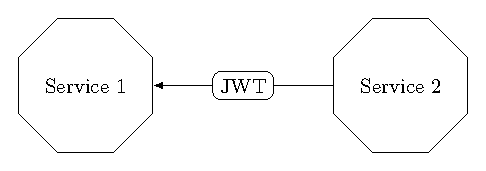
\includegraphics{images/authentication-mechanisms/TikZ_jwt_base_structure.pdf}
	\caption{Setup using self signed JWTs for the service-to-service authentication~\cite{dias2020microservices}}
	\label{fig:auth_mechanisms_jwt}
\end{figure}

The usage of self-signed JWTs does not provide any confidentiality for the communication among the services.
Therefore TLS should be used to secure service-to-service communication.
Since the authentication is not dependent on TLS, it is possible to use other mechanisms instead of TLS.
For example, JSON Web Encryption or any other encryption mechanism can be used, but usually, it does not make sense to exchange TLS~\cite{dias2020microservices}.

The usage of self-signed JWTs additionally provides non-reputability.
This means each action is bound to the service that created the JWT, and the service can not repudiate that the JWT was created by him~\cite{dias2020microservices}.
Whenever non-reputability is a requirement of the system, self-signed JWTs are the superior authentication mechanism.

\subsection{Non Repudability}
Digital signatures can be used to achieve non-reputability cryptographically.
This means that when one service acts as another service, the receiving service can prove that the calling service initiated the action.
A practical example is that a customer creates an order consuming the "OrderService" and the "OrderService" updates the inventory using the "InventoryService".
The "InventoryService" could save the JWT it received from the "OrderService".
The "InventoryService" can later prove that the update was initiated by the "OrderService" because only the "OrderService" could have created the JWT with a valid signature.
Therefore each transaction within the deployment can be comprehended entirely, as long as the services store the received JWTs~\cite{dias2020microservices}.

Nonrepudability and authentication are very similar.
Authentication is about convincing the other party that an event is valid.
With nonrepudiation, it is even possible to prove the truth of an event to a third party~\cite{wu20131200}.

\subsection{Passing the end-user context}
The approaches to how the end-user context is passed between the services are similar to the approaches explained in~\ref{sec:mtls_end_user_context}.
The big difference is how the JWT is transferred among the services.
While with mTLS, the JWT was embedded within the body or as a URL parameter, with self-signed JWTs, it can be embedded within the JWT that already has to be transferred.
This is done by appending a nested JWT within the claims of the self-signed JWT.
The signature of the JWT, which is used for authentication, can still be verified by using the service's public key.
Nevertheless, the signature of the nested JWT is verified using the public key of the STS.
This means the JWT is carried in a way that can not be forged.
Therefore it is better to use self-signed JWTs for the authentication when the end-user context is relevant in many situations~\cite{dias2020microservices}.

\subsection{Conclusion}
service-to-service authentication using self-signed JWTs is not only a mechanism for authentication. It additionally provides nonrepudiation and makes sharing the user context more convenient. 
Otherwise, the implementation of self-signed JWTs is much more challenging than the implementation of mTLS.
It is insufficient to configure the webserver correctly and append a certificate to each request.
Every service has to know how to encode and decode JWTs unless he only sends or receives requests.
Furthermore, to achieve nonrepudiation, all received JWTs must be stored for an adequate timespan, requiring additional database storage.

One major advantage is that the authentication using self-signed JWTs can be implemented differently.
It does not matter which technology is used to provide confidentiality for the communication among the services.
The common way is TLS, and there are not many reasons to get rid of TLS, but the fact that it is possible to get rid of TLS can be an advantage in some situations.
It does not matter which technology is used to transfer the public key of the sending service to the receiving service.
Moreover, the developers can vary some other parameters, which is not possible using mTLS because it is a strictly defined protocol.

Sadly the biggest challenge of mTLS, which is the key management, can not be avoided using self-signed JWTs, because it also requires each service to have its key pair.
Nevertheless, the key management can be simplified since it is unnecessary to have a CA responsible for signing each certificate.
Still, regarding the webserver setup, it makes sense to have one superior authority, that is, the root of trust and whose chained certificates are trusted.

As a result, self-signed JWTs are the preferred authentication mechanism when the target is to achieve nonrepudiation or when the system is very dependent on sharing the user context.
Nevertheless, this leads to additional implementation overhead and requires developers who specialize in security-related systems.
